\section{Discussion and outlook}%
\label{sec:result_discussion}

The results obtained as part of the searches for non-resonant SM \HH
production and resonant production via narrow width scalar bosons are
discussed in the following.

Both searches are largely limited by data statistical uncertainties
which represent the majority of the uncertainty on extracted signal
strengths or cross sections. Systematic uncertainties are
comparatively small for the search for non-resonant SM \HH production
and resonant production at intermediate to high masses. Only for the
search for low mass scalar resonances uncertainties from systematic
sources are comparable to data statistical uncertainties, however,
they do not solely limit the final result.

Thus the largest improvements are expected from increases in the
integrated luminosity expected for Run~3 of the LHC and beyond. The
prospects of searches for Higgs boson pairs for Run~4 (high luminosity
LHC) studied by the ATLAS collaboration
in~\cite{ATL-PHYS-PUB-2022-005} are briefly discussed providing an
outlook for future searches.

% Or by further relaxing the selection requirements yielding larger
% signal acceptance. Although this would also increase the background
% and thus might not correspond to a net improvement of the results.

\subsection{Search for non-resonant production of Higgs boson pairs}

\begin{figure}[htbp]
  \centering

  \begin{subfigure}{0.53\textwidth}
    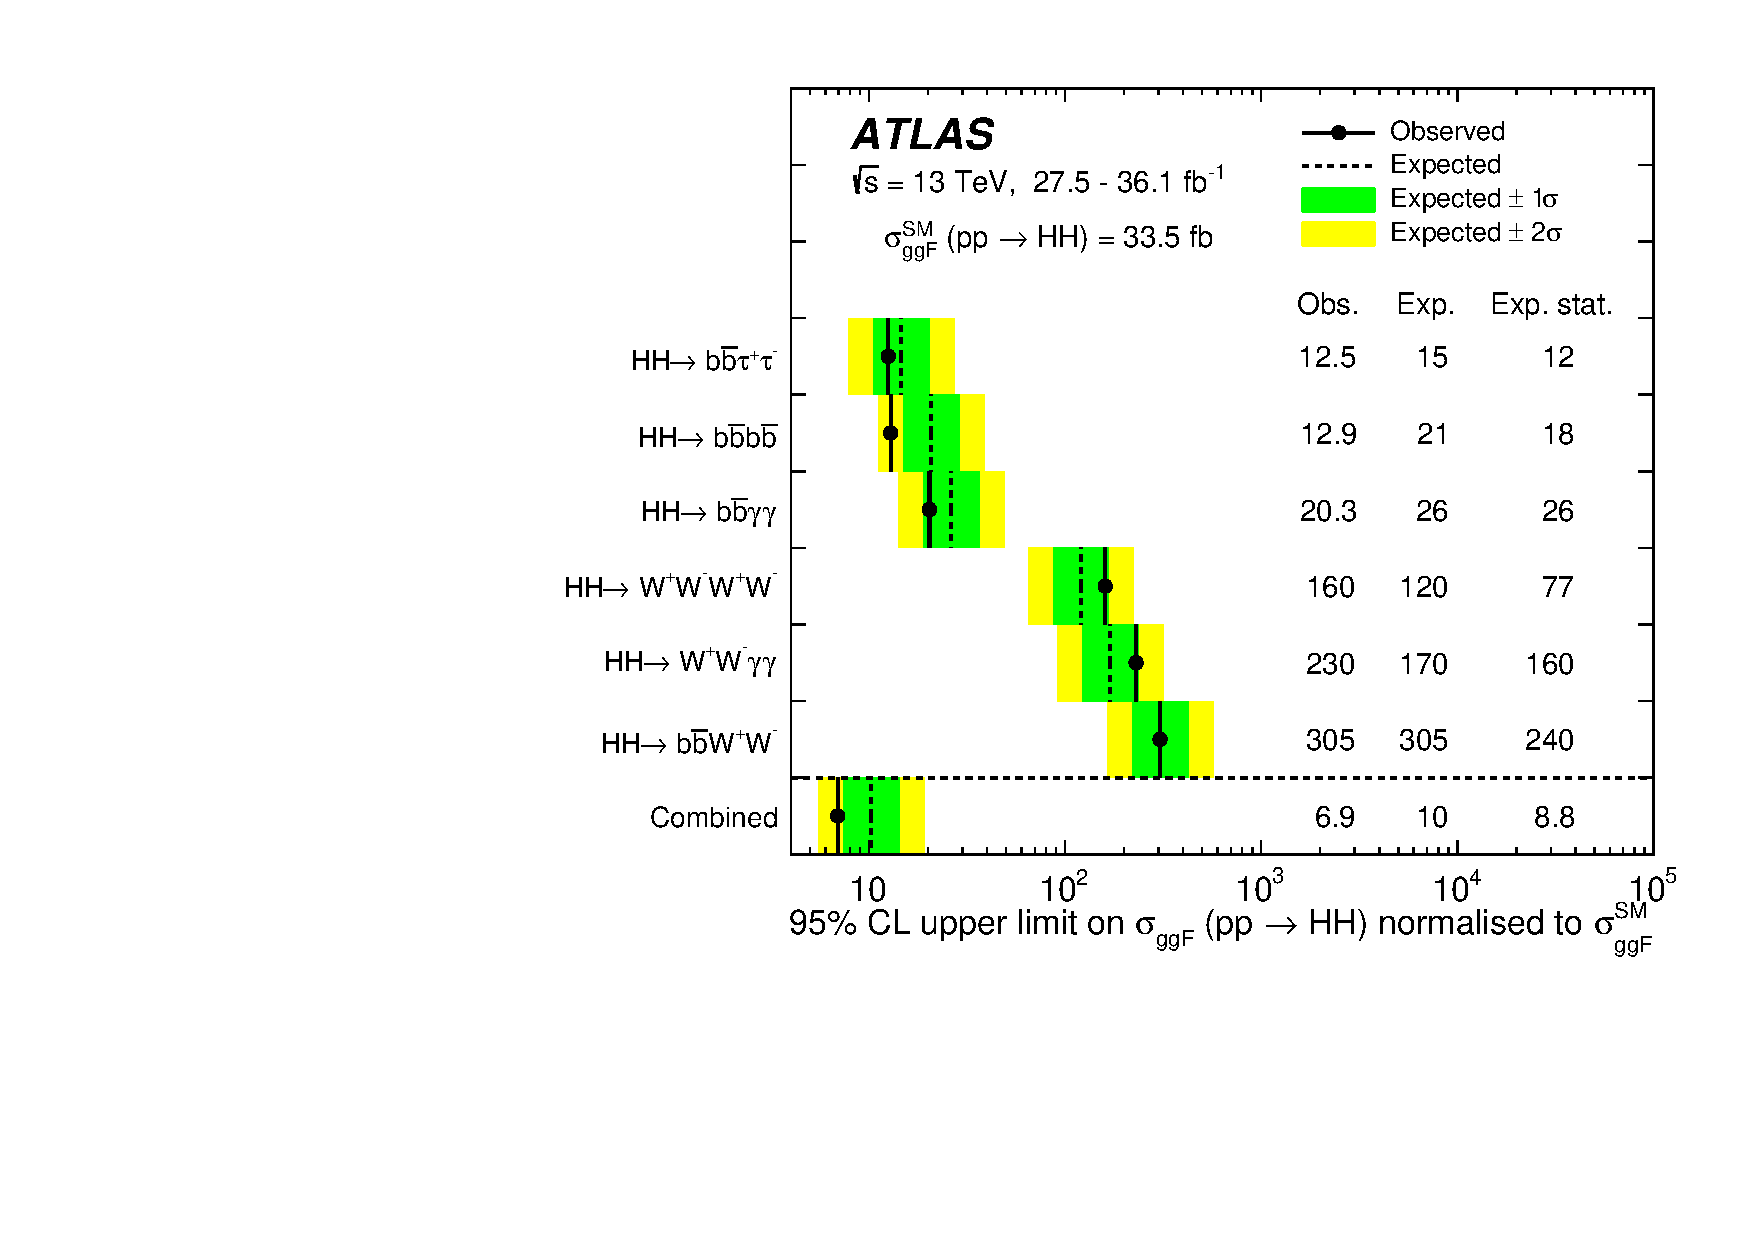
\includegraphics[width=\textwidth]{discussion/results_36ifb}
    \subcaption{Partial Run~2 dataset with an integrated luminosity of \num{27.5} -
      \SI{36.1}{\per\femto\barn}~\cite{HDBS-2018-58}}
  \end{subfigure}\hfill%
  \begin{subfigure}{0.45\textwidth}
    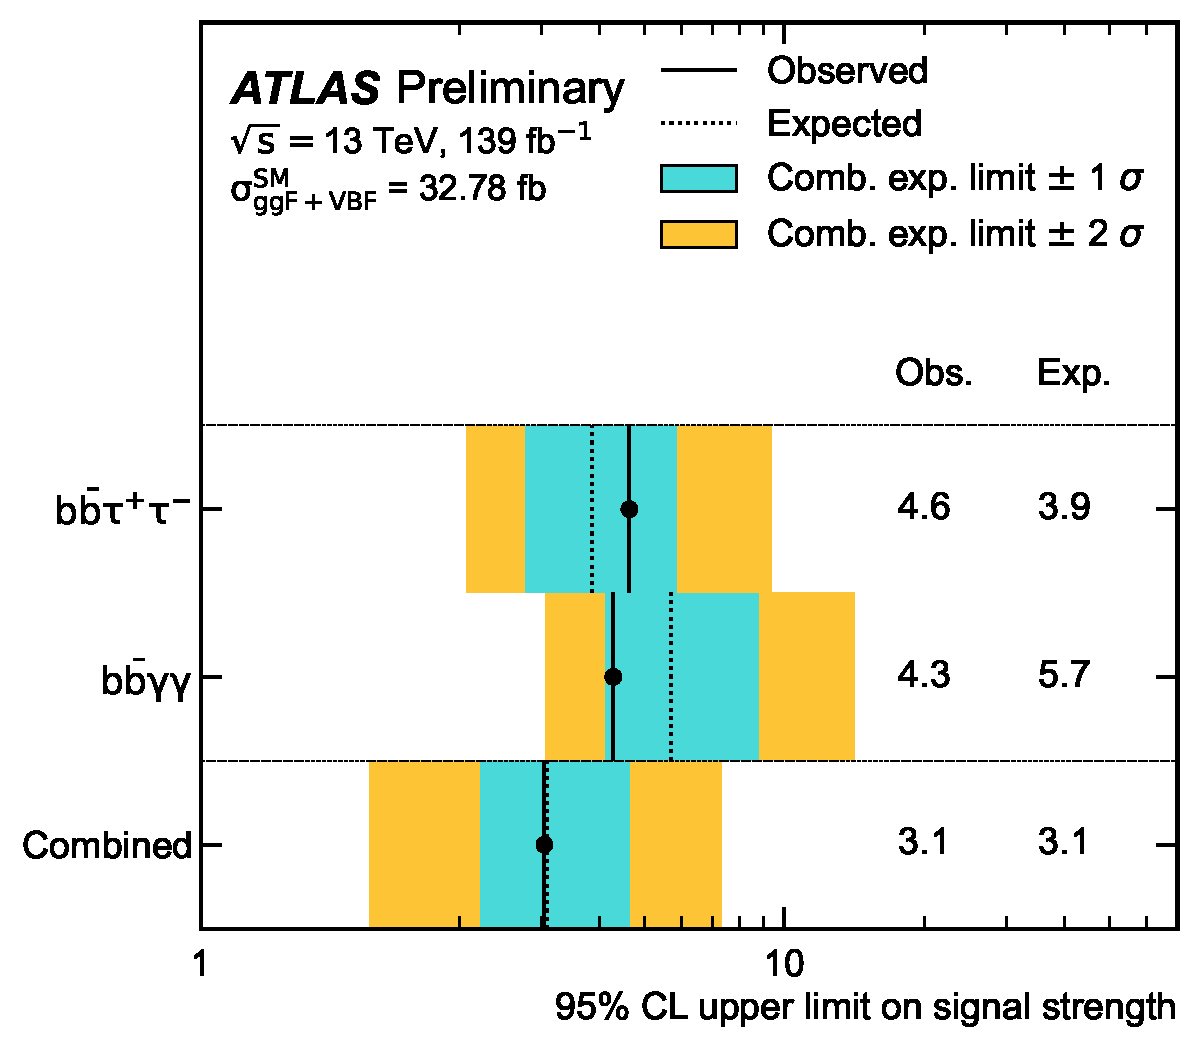
\includegraphics[width=\textwidth]{discussion/results_139ifb}
    \subcaption[margin=5em]{Full Run~2 dataset with an integrated luminosity
      of~\SI{139}{\per\femto\barn}~\cite{ATLAS-CONF-2021-052}}
  \end{subfigure}

  \caption{Comparison of ATLAS results for searches for non-resonant
    SM \HH production from the beginning (a) and end of Run~2 (b) of
    the LHC. Upper limits are shown in terms of the signal strength of
    SM \HH production via \ggF neglecting the VBF production mode in
    (a) and in terms of the combined signal strength of \ggF and VBF
    production mode in (b). Both results are still comparable due to
    the small cross section of VBF \HH production. Addtionally, the
    assumed SM \HH cross sections changed between results due to the
    availability of improved theoretical predictions.  Note the
    different results for bbtautau. }
  \label{fig:atlas_run2_hh_results}
  \todo[inline]{Make my own plot / table for RHS including bbWW and
    possibly 4b? 4b obs.\ 5.4 (exp.\ 8.1)}
\end{figure}

Comparison of early with full Run~2 results. Expectation from
luminosity scaling. Comparison with extrapolations from early Run~2
data.

The improvement in the analysis can be seen when performing an
approximate extrapolation of the ATLAS result with
\SI{36.1}{\per\femto\barn} integrated luminosity and an expected upper
limit on $\mu$, assuming that the result is limited by the data
statistical sources, to the integrated luminosity of the $pp$ dataset
at the end of Run~2. Extrapolating the expected upper limit to the
integrated luminosity of \SI{139}{\per\femto\barn} yields a limit of
the signal strength of about 7

% \footnote{A pessimistic bound on the
%   relative change of \SI{95}{\percent} CL upper limits is given by
%   $\sqrt{\mathcal{L}_1 / \mathcal{L}_2$.}.


The upper limit at \SI{95}{\percent}

\todo[inline]{Improvements with respect to the previous
  analysis. Outscaling lumi...}

\todo[inline]{Major improvements from: Improvements in b-tagging, tau
  reconstruction and tau-id.}

Comparison with CMS results.

\begin{table}[htbp]
  \centering

  \begin{tabular}{l@{\hskip 2em}SSc}
  \toprule
  \textbf{CMS} (\SI{138}{\per\femto\barn}) & \multicolumn{3}{c}{Upper limit on $\mu_{gg\text{F+VBF}}$ (\SI{95}{\percent} CL)} \\
  \cmidrule{2-4}
  Final state & {Observed} & {Expected} & Reference \\
  \midrule
  $\bbbar\tau^{+}\tau^{-}$ & 3.3 & 5.2 & \cite{CMS-PAS-HIG-20-010} \\
  $\bbbar\gamma\gamma$ & 7.7 & 5.2 & \cite{CMS-HIG-19-018} \\
  $\bbbar\bbbar$ & 3.9 & 7.8 & \cite{CMS-HIG-20-005-PREPRINT} \\
  % Multilepton = ($W^+W^-W^+W^-$, $W^+W^-\tau^+\tau-$, $\tau^+\tau^-\tau^+\tau^-$)
  Multi-lepton  & 21.8 & 19.6 & \cite{CMS-PAS-HIG-21-002} \\
  \bottomrule
\end{tabular}


%%% Local Variables:
%%% mode: latex
%%% TeX-master: "../phd_thesis"
%%% End:


  \caption{Table of CMS results of searches for non-resonant
    production of Higgs boson pairs with an integrated luminosity of
    \SI{138}{\per\femto\barn}. Upper limits are shown at
    \SI{95}{\percent} CL on the signal strength of the combination of
    the \ggF and VBF production modes.}
  \label{tab:cms_nonresonant}
\end{table}


\begin{itemize}
\item Why is hadhad more sensitive?
\end{itemize}

\todo[inline]{This analysis yields the best expected sensitivity to
  the SM Higgs boson pair production.}



Previous extrapolation~\cite{ATL-PHYS-PUB-2018-053}

bbtautau extrapolation for HL-LHC ($\sqrt{s} = \SI{14}{\TeV}$):
\cite{ATL-PHYS-PUB-2021-044}
\begin{itemize}
\item Expected statistical significance of $2.8\,\sigma$ using
  best-guess assumptions regarding the evolution of systematic
  uncertainties going from Run~2 to Run~4 of the LHC.
\end{itemize}


\subsection{Search for resonant production of Higgs boson pairs}

How does the excess fit into other results?

$4b$: \SI{6.5}{\femto\barn} (exp.\ \SIpmerr{8.15}{+1.17}{-0.77}{\femto\barn})

\todo[inline]{Discussion excess: Modelling of collinear taus?}


%%% Local Variables:
%%% mode: latex
%%% TeX-master: "../../phd_thesis"
%%% End:
